\documentclass[11pt]{amsart}
\usepackage[margin=1.05in]{geometry}
\usepackage{amsmath,amssymb,amsthm,mathtools}
\usepackage{booktabs}
\usepackage{array}
\usepackage{graphicx}
\usepackage{tikz}
\usepackage{xcolor}
\usepackage{xr-hyper}
\usepackage[hidelinks]{hyperref}
\usepackage{url}
\usepackage{xurl}
\usepackage[T1]{fontenc}
\newcommand{\lr}{\ell}
\newcommand{\pp}{p}
\newcommand{\GEN}{\mathrm{GEN}}
\newcommand{\RAD}{\mathrm{RAD}}
\newcommand{\ROOT}{\mathrm{ROOT}}
\externaldocument[][nocite]{main}
\makeatletter
\@for\@tempa:=-1,0,1,2,3\do{%
  \expandafter\gdef\csname r@tocindent\@tempa\endcsname{0pt}}%
\makeatother
\sloppy
\allowdisplaybreaks

\newtheorem{theorem}{Theorem}[section]
\newtheorem{proposition}[theorem]{Proposition}
\newtheorem{lemma}[theorem]{Lemma}
\newtheorem{corollary}[theorem]{Corollary}
\newtheorem{conjecture}[theorem]{Conjecture}
\theoremstyle{definition}
\newtheorem{definition}[theorem]{Definition}
\theoremstyle{remark}
\newtheorem{remark}[theorem]{Remark}
\newtheorem{example}[theorem]{Example}

\title[Supplement]{Supplement to Induced Paths, Radius, and Extremal Neighborhood Independence in Graphs without 4-Cycles}
\author{Xingchen Wang}
\author{Neil Xu}
\date{November 2026}

\begin{document}
\maketitle

\begin{abstract}
This supplement contains the rooted bounds, the endpoint obstructions, the high-radius constructions, and the conditional reduction for $\GEN_3$ removed from the article. Numbered references to results proved in the article point to that file. The article's Theorems on $M(n)$, radius four, the exact triangle-free function $f(n)$, and graphs with at most one triangle do not depend on these arguments.
\end{abstract}

\section{Rooted bounds of orders three and four}\label{sec:root3}

The arguments of this section and of Sections~\ref{sec:blocks} and~\ref{sec:neg} are not used for Theorems~\ref{thm:petersen}, \ref{thm:r4}, \ref{thm:tf}, \ref{thm:fn} and~\ref{thm:onetri} or for Corollary~\ref{cor:cellsharp}. The rooted bound that bears on the next open band is Theorem~\ref{thm:root4}: it is the estimate which shows that a minimum counterexample to $\GEN_4$ is $2$-connected. The distance-layer form of the same estimate is omitted. The block-class bound and the Moore observation are kept because they delimit $\GEN_K$, and Example~\ref{ex:ep} is kept because it is the explicit failure of the endpoint inequalities at order nine.

For a vertex $s$ of a connected graph $F$ let $\pp_s(F)$ be the largest order of an induced path starting at $s$. Write $D=d_F(s)$ and $m=e(F[N(s)])$.

\begin{definition}\label{def:root}
For an integer $q\ge 3$, the rooted bound $\ROOT(q)$ asserts that every connected strong $C_4$-free graph $F$ and every vertex $s$ with $\pp_s(F)\le q$ satisfy
\[
S(F)\le(q-1)(|F|-1)-(q-3)D-m.
\]
\end{definition}

The hypothesis $\pp_s(F)\le q$ belongs in the statement. Without it the displayed inequality is false: if $q=3$ and $F=C_5$, then $S(F)=10$ and $m=0$, while $2(|F|-1)=8$. Lemma~\ref{lem:rootedp4}, already proved because the cut-vertex induction of Theorem~\ref{thm:tf} uses it, is the case $q=3$.

\begin{theorem}\label{thm:root4}
Let $F$ be connected and strong $C_4$-free, and let $s\in V(F)$ satisfy $\pp_s(F)\le 4$. Write $D=d(s)$ and $m=e(F[N(s)])$. Then
\begin{equation}\label{eq:root4}
S(F)\le 3(n-1)-D-m.
\end{equation}
In particular $\ROOT(4)$ holds. Equality holds for $C_5$ at any root, and for a graph formed by $k\ge 1$ copies of $C_5$ that meet only at the root.
\end{theorem}

\begin{figure}[htbp]
  \centering
  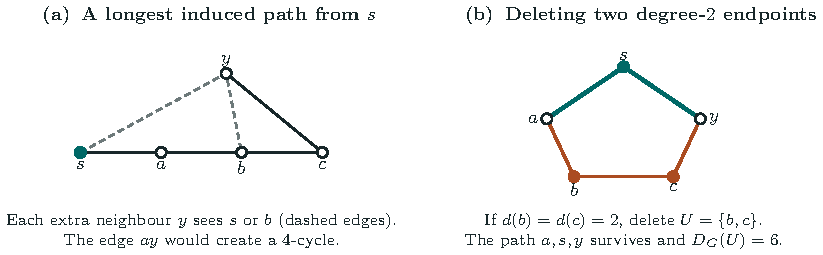
\includegraphics[width=.98\linewidth]{fig3-root4.pdf}
  \caption{Deletion at the end of a longest induced path of order four
    starting at $s$. (a) Each neighbor $y\ne b$ of $c$ must be adjacent to
    $s$ or $b$. Dashed lines indicate alternatives. (b) If neither terminal
    vertex $c$ nor $b$ can be deleted with loss at most three, the indicated
    $5$-cycle is induced and both have degree two. The deletion of
    $\{b,c\}$ has loss six and preserves connectivity.}
  \label{fig:root-four}
\end{figure}

\begin{proof}
The proof is by induction on $n$. If $\pp_s(F)\le 3$, Lemma~\ref{lem:rootedp4} gives $S\le 2(n-1)-m$. Since $D\le n-1$, the right-hand side is at most $3(n-1)-D-m$.

Now suppose $\pp_s(F)=4$, and let $s,a,b,c$ be an induced path. The endpoint $c$ is not a cut vertex: a neighbour of $c$ in a component of $F-c$ that does not contain $s$ would extend the path. Let $y\in N(c)\setminus\{b\}$. The path $s,a,b,c,y$ is not induced, so $y$ meets at least one of $s,a,b$. The edge $ya$ would give the $4$-cycle $a,b,c,y$. Thus $y$ is adjacent to $s$ or to $b$. The vertices $s$ and $c$ have at most one common neighbour, and so do $b$ and $c$, hence $d(c)\le 3$. If $d(c)=3$, then $c$ has two neighbours besides $b$, and one of them is adjacent to $b$. So $c$ lies in a triangle, $t(c)\ge 1$ and $L(c)=2d(c)-3t(c)\le 3$. Figure~\ref{fig:root-four} shows the two deletions.

If $L(c)\le 3$, delete $c$. The graph $F-c$ is connected, and $c\notin N[s]$, so $D$ and $m$ are unchanged. The inductive hypothesis gives $S(F-c)\le 3(n-2)-D-m$, and therefore $S(F)\le 3(n-2)-D-m+3=3(n-1)-D-m$.

The remaining case is $d(c)=2$ and $t(c)=0$, so $L(c)=4$. Let $y$ be the neighbour of $c$ other than $b$. Then $y$ is not adjacent to $b$, hence $ys$ is an edge, and $s,a,b,c,y$ is an induced $5$-cycle: every chord is excluded by the induced path $s,a,b,c$, by $t(c)=0$, or by the $4$-cycle that $ay$ would create. The vertex $b$ is the endpoint of the induced path $s,y,c,b$. If $L(b)\le 3$, delete $b$ and apply the inductive hypothesis as above.

Otherwise the same endpoint analysis gives $d(b)=2$ and $t(b)=0$. Delete $U=\{b,c\}$. A path that used the edges $ab,bc,cy$ can be replaced along $a,s,y$, so $F-U$ is connected. The deleted edges are $ab$, $bc$ and $cy$, and no triangle is deleted. Since $S=2e-3T$, one has $D_F(U)=6=3|U|$. The vertices $b$ and $c$ lie outside $N[s]$, so $D$ and $m$ are unchanged. Induction gives $S(F-U)\le 3(n-3)-D-m$, and $S(F)\le 3(n-3)-D-m+6=3(n-1)-D-m$.

For the equality examples, root $C_5$ at any vertex. Then $n=5$, $D=2$, $m=0$ and $S=10=3(n-1)-D-m$. If $k$ copies of $C_5$ meet only at the root, then $n=1+4k$, $D=2k$ and $m=0$, because the two neighbours of the root on each copy are nonadjacent, and $S=10k=3(n-1)-D-m$.
\end{proof}

\begin{proposition}\label{prop:root4plus}
Let $F$ be connected and strong $C_4$-free, and let $s$ satisfy $\pp_s(F)=4$ and $\mathrm{ecc}(s)=3$. Then $S(F)\le 3(n-1)-D-m-2$. Equality holds for $P_4$ rooted at an endpoint.
\end{proposition}

\begin{proof}
The proof is by induction on $n$ for instances with $\pp_s=4$ and $\mathrm{ecc}(s)=3$. Fix a vertex $z$ at distance $3$ from $s$. Whenever an endpoint other than $z$ exists, the deletion in the proof of Theorem~\ref{thm:root4} applies to it. In the exceptional $5$-cycle the vertices $b$ and $c$ are at distance $2$ from $s$, so the deletion leaves $z$. The remaining graph is connected and strong $C_4$-free, $D$ and $m$ are unchanged, and distances do not decrease. Thus $d(s,z)\ge 3$. Since $\pp_s\le 4$, no distance exceeds $3$, so $\pp_s=4$ and the eccentricity of $s$ is still $3$. A deletion of one vertex of loss at most~$3$ contributes $3$, and the inductive bound on $n-1$ vertices contributes $3(n-2)-D-m-2$, which sum to $3(n-1)-D-m-2$. Deleting $\{b,c\}$ contributes $6$ against $3(n-3)-D-m-2$.

If $z$ is the unique endpoint, delete $z$. Then $\pp_s(F-z)\le 3$. An extra neighbour of $z$ is not adjacent to $s$, for that would give $d(s,z)\le 2$. By the endpoint analysis it is adjacent to the predecessor of $z$ and forms a triangle, so $L(z)\le 2$. Lemma~\ref{lem:rootedp4} gives $S(F-z)\le 2(n-2)-m$, hence $S(F)\le 2(n-1)-m$. A geodesic from $s$ to $z$ has at least two vertices outside $N[s]$, so $n-1-D\ge 2$ and $2(n-1)-m\le 3(n-1)-D-m-2$.

For $P_4$ rooted at an endpoint one has $n=4$, $D=1$, $m=0$ and $S=6$, and the strengthened bound is $3\cdot 3-1-2=6$.
\end{proof}

\begin{proposition}\label{prop:gen4cut}
Let $G$ be a counterexample to $\GEN_4$ of minimum order. Then $G$ is $2$-connected. This does not decide $\GEN_4$.
\end{proposition}

\begin{proof}
Such a graph is connected and strong $C_4$-free, with $\pp(G)\le 8$ and $S(G)\ge 4n+1$. Let $v$ be a cut vertex, and let $G_1,G_2$ be the graphs of Lemma~\ref{lem:cut}. Write $\rho_i$ for the largest order of an induced path of $G_i$ that starts at $v$. Paths from the two sides form an induced path of $G$ on $\rho_1+\rho_2-1\le 8$ vertices, so some side, say $G_1$, has $\rho_1\le 4$. Theorem~\ref{thm:root4} gives $S(G_1)\le 3(n_1-1)$. The graph $G_2$ is a smaller connected strong $C_4$-free graph of path order at most~$8$, so minimality gives $S(G_2)\le 4n_2$. Therefore $S(G)\le 3(n_1-1)+4n_2$. Since $n=n_1+n_2-1$,
\[
3(n_1-1)+4n_2=4n-n_1+1.
\]
The hypothesis $n_1\ge 2$ gives $4n-n_1+1\le 4n-1$, so $S(G)<4n$, contradicting $S(G)\ge 4n+1$.
\end{proof}

For $q\ge 5$ the bound $\ROOT(q)$ is not proved for arbitrary strong $C_4$-free graphs. Section~\ref{sec:status} records the limitation. The next section proves every index for graphs whose blocks are bipartite or cycles. Conjecture~\ref{conj:td} would imply $\ROOT(q)$ for the same $q$, by the attachment in Section~\ref{sec:status}. That implication is not a proof of the conjecture, and for $q\ge 5$ it does not prove $\ROOT(q)$.

\section{Rooted bounds for every index}\label{sec:blocks}

Let $\mathcal B$ be the class of connected strong $C_4$-free graphs in which every block is bipartite or a cycle. Edges are blocks, and cycles may be odd. The class contains every connected strong $C_4$-free bipartite graph and every connected strong $C_4$-free cactus. Theorem~\ref{thm:blocks} keeps this block hypothesis. The graph $K_{2,3}$ does not show that the hypothesis is necessary. Its only block is itself, and that block is bipartite, but $K_{2,3}$ contains a $4$-cycle subgraph. Rooted in its part of size two it has $\pp_s=3$ and $S=12>2(n-1)-m=8$. The example tests the failure of $\ROOT(3)$ after the strong $C_4$-free hypothesis is removed. It does not test the block restriction inside the strong $C_4$-free class.

A rooted graph $(G,s)$ with $\pp_s(G)=q$ and $\mathrm{ecc}(s)=q-1$ is called \emph{terminal}. For a terminal instance put $R=n-q+1-D\ge 0$, the number of vertices outside $N[s]$ and outside a root-to-farthest-vertex geodesic. Set $c_2=0$, $c_3=2$, $c_4=3$ and $c_q=2\lfloor(q-1)/2\rfloor$ for $q\ge 5$.

\begin{lemma}\label{lem:blockdeg}
Let $G$ be connected and strong $C_4$-free, and let $P$ be a longest induced path starting at a vertex $s$, of order $q$. Let $x$ be the other end of $P$, and suppose that the block $B$ containing $x$ is bipartite. Let $Q$ be the subpath of $P$ formed by the vertices of $P$ that lie in $B$, and set $\ell=|Q|$. Then every neighbour of $x$ lies in $B$, and $x$ lies in no triangle. If $\ell=2$, then $d(x)=1$. If $\ell\ge 3$, then $d(x)\le\lfloor(\ell-1)/2\rfloor$. In every case $\ell\le q$, and $L(x)\le c_q$ whenever $q\ge 5$.
\end{lemma}

\begin{proof}
A neighbour of $x$ in a component of $G-x$ that does not contain $s$ would extend $P$, so $x$ is not a cut vertex. Every edge with one end in $B$ and one end outside $B$ is incident with a cut vertex of $B$. Therefore every neighbour of $x$ lies in $B$. The block is bipartite, so $x$ lies in no triangle.

Since the block-cut tree is a tree, $P$ enters $B$ only once. The intersection of $P$ with $B$ is a single subpath $Q=z_0,\dots,z_{\ell-1}$ with $z_{\ell-1}=x$. If $s$ lies in $B$, then $Q=P$. If $s$ lies outside $B$, the vertices of $P$ that precede $z_0$ lie outside $B$, and $z_0$ is their only neighbour in $B$: any other edge from that prefix into $B$ would be a second entry. A vertex of $B\setminus\{z_0\}$ is therefore adjacent to no vertex of the prefix. An extension of $P$ at $x$ through a vertex of $B$ can fail only by a chord into $Q$.

Let $y$ be a neighbour of $x$ other than $z_{\ell-2}$. Then $y$ lies in $B$, and $y$ does not lie on $Q$, because $Q$ is induced. The vertex $y$ is not adjacent to the prefix. If $y$ had no neighbour on $Q$, the path $P$ followed by $y$ would be induced. Thus $y$ has a neighbour $z_i$ on $Q$. This neighbour is not $x$. It is not $z_{\ell-2}$, for $yxz_{\ell-2}$ would be a triangle, and it is not $z_{\ell-3}$, for $z_{\ell-3}z_{\ell-2}xy$ would be a $4$-cycle. Since $B$ is bipartite, $z_i$ has the colour of $x$, so $i\equiv\ell-1\pmod 2$ and $i\le\ell-5$.

If $\ell=2$, then $Q$ is a single edge and there is no admissible index, so $d(x)=1$. If $\ell\ge 3$, the number of admissible indices is $\lfloor(\ell-1)/2\rfloor-1$. Two neighbours of $x$ are nonadjacent and cannot share a blocker, for a common blocker would form a $4$-cycle with them and with $x$. Hence $d(x)\le\lfloor(\ell-1)/2\rfloor$. In every case $\ell\le q$. For $q\ge 5$ one has $d(x)\le\lfloor(q-1)/2\rfloor$, and $L(x)=2d(x)\le c_q$.

The same count applies inside $B$. Let $z$ be the cut vertex of $B$ lying on every path from a fixed root to $B$, or the root itself if the root lies in $B$, and let $Q$ be a longest induced path of $B$ starting at $z$, with other end $x$ and with $\ell=|Q|$. A neighbour of $x$ in $B$ that had no neighbour on $Q$ would extend $Q$ inside $B$. If the root lies outside $B$, no vertex of $B\setminus\{z\}$ meets the component of the root at $z$, so that component contributes no further blocker. Thus $d_B(x)\le 1$ if $\ell=2$, and $d_B(x)\le\lfloor(\ell-1)/2\rfloor$ if $\ell\ge 3$.
\end{proof}

\begin{theorem}\label{thm:blocks}
\begin{enumerate}
\item Every terminal instance in $\mathcal B$ satisfies $S(G)\le 2(D+q-2)-m+c_q R$.
\item Every $F\in\mathcal B$ with a vertex $s$ such that $\pp_s(F)\le q$ satisfies
\[
S(F)\le c_q(n-1)-(c_q-2)D-m.
\]
In particular $\ROOT(q)$ holds in $\mathcal B$ for every $q\ge 3$. If every block is bipartite or a triangle, one may take $c_q=2\lfloor(q-1)/2\rfloor$ for all $q\ge 3$.
\end{enumerate}
\end{theorem}

\begin{proof}
\emph{Two terminal facts.} An endpoint $x$ of a longest rooted induced path is not a cut vertex: a neighbour of $x$ in another component of $G-x$ would extend the path. If $z$ is at distance $q-1$ from $s$ and $v_0=s,\dots,v_{q-1}=z$ is a geodesic, any neighbour $y\ne v_{q-2}$ of $z$ must meet an earlier path vertex (else the rooted path extends); meeting $v_i$ with $i\le q-4$ shortens $d(s,z)$, and meeting $v_{q-3}$ gives a $C_4$; so $y\sim v_{q-2}$, and two such $y$ would give a $C_4$. Hence $L(z)=2d(z)-3t(z)\le 2$. Moreover, if $x\ne s,z$, $G-x$ is connected and $z$ survives, then $q-1\le d_{G-x}(s,z)\le\pp_s(G-x)-1\le q-1$, so the instance stays terminal with the same $q$.

\emph{Endpoint losses.} Let $x$ be the endpoint of a longest rooted path of order $q$. It lies in a single block. If that block is a triangle the loss $L(x)$ is $1$, if an edge $2$, and if a cycle of length at least $5$ it is $4$. If the block is bipartite, Lemma~\ref{lem:blockdeg} gives $L(x)\le c_q$ for $q\ge 5$.

\emph{No nontrivial bipartite block when $q\le 4$.} Let $B$ be a nontrivial bipartite block, and let $z$ be the cut vertex of $B$ that lies on every path from $s$ to $B$, or let $z=s$ if $s\in B$. Let $Q$ be a longest induced path of $B$ starting at $z$, and let $x$ be its other end. Every vertex of a nontrivial block has degree at least two in the block, so $d_B(x)\ge 2$. The last paragraph of Lemma~\ref{lem:blockdeg} gives $d_B(x)\le 1$ if $|Q|\le 4$ and $d_B(x)\le\lfloor(|Q|-1)/2\rfloor$ in any case with $|Q|\ge 3$. The inequality $d_B(x)\ge 2$ therefore forces $|Q|\ge 5$. An induced $s$--$z$ path meets $B$ only at $z$. Concatenating it with $Q$ yields an induced path that starts at $s$. The order of this path is $|Q|$ if $s\in B$, and at least $|Q|+1$ if $s\notin B$. In either case $\pp_s(G)\ge 5$. A terminal instance with $q\le 4$ therefore has no nontrivial bipartite block. Every block is an edge, a triangle, or a cycle of length at least five, so the graph is a cactus.

\emph{Bases.} For $q\le 4$ the preceding paragraph leaves only cacti. For a $C_4$-free cactus with $c_3$ triangle blocks and $c_L$ longer cycle blocks, $S=2(n-1)+2c_L-c_3$ and $m\le c_3$. For $q=3$ no longer cycle occurs, and (1) follows. For $q=4$ every longer cycle is a $C_5$ through $s$. A chosen length-$3$ geodesic uses at most one edge of each such $C_5$: if it used two edges and then left the cycle, replacing that two-edge arc by the other three-edge arc would give an induced rooted path of order $5$. So each $C_5$ contributes two vertices to $R$, $R\ge 2c_L$, and $[2(D+2)-m+3R]-S=R-2c_L+c_3-m\ge 0$. For $q=2$ the root is universal and $S=2D-m$.

\emph{Induction on $n$.} Let $E$ be the set of endpoints of rooted induced paths of order $q$ and $z$ a farthest vertex, so $z\in E$. If some $x\in E\setminus\{z\}$ exists, delete it: $x\notin N[s]$, $x$ is not a cut vertex, its loss is at most $c_q$, the instance remains terminal with the same $q$, $D$ and $m$, and $R$ drops by one. If $E=\{z\}$, delete $z$: the new rooted maximum is $q-1$, the eccentricity $q-2$, $R$ is unchanged and the loss is at most $2$; induction gives $S\le 2(D+q-3)-m+c_{q-1}R+2\le 2(D+q-2)-m+c_q R$. Deletion preserves membership in $\mathcal B$. This proves (1); the bipartite-or-triangle variant is identical.

(2) Attach a new path with $q-1$ edges at $s$. The result is terminal of index $q$, lies in $\mathcal B$, has order $n+q-1$, mass $S+2(q-1)$ and root degree $D+1$, and $m$ is unchanged. Substituting into (1) gives (2). Since $c_q\le q-1$ and $n-1-D\ge 0$,
\begin{align*}
c_q(n-1)-(c_q-2)D-m
&=c_q(n-1-D)+2D-m\\
&\le(q-1)(n-1-D)+2D-m\\
&=(q-1)(n-1)-(q-3)D-m,
\end{align*}
so $\ROOT(q)$ follows.
\end{proof}

A matching upper bound of shape $S\le(r-1)n-2r(r-3)$, for graphs in $\mathcal B$ of radius $r\ge 5$ and path order $2r-1$, has been proposed from a structural description of radius-extremal graphs. That description is not proved in this paper, and the radius bound in $\mathcal B$ is not claimed.

\begin{lemma}\label{lem:blockers}
Let $G$ be strong $C_4$-free and triangle-free, and let $x_0x_1\cdots x_k$ be an induced path that cannot be extended at $x_k$. If $d(x_k)\ge 2$, then $k\ge d(x_k)+1$. If moreover $G$ is bipartite, then $k\ge 2d(x_k)$.
\end{lemma}

\begin{proof}
Let $y\ne x_{k-1}$ be a neighbour of $x_k$. It is not on the path, and, since the path cannot be extended, $y$ has a neighbour $x_i$ with $i\le k-1$. Here $i\ne k-1$ (a triangle) and $i\ne k-2$ (the $4$-cycle $x_{k-2}x_{k-1}x_ky$), so $i\le k-3$. A vertex $x_i$ is adjacent to at most one neighbour of $x_k$. Hence the $d(x_k)-1\ge 1$ such neighbours need distinct blockers among $x_0,\dots,x_{k-3}$, and $k-2\ge d(x_k)-1$. If $G$ is bipartite, the blocker has the colour of $x_k$, so $i\equiv k\pmod 2$ and $i\le k-4$; there are $\lfloor k/2\rfloor-1$ such positions, and $\lfloor k/2\rfloor\ge d(x_k)$.
\end{proof}

\begin{proposition}\label{prop:regbip}
Every connected regular bipartite strong $C_4$-free graph satisfies $\GEN_K$ for every $K$ and satisfies REAL-133. Every Moore graph of diameter~$2$ and girth~$5$ satisfies REAL-133.
\end{proposition}

\begin{proof}
Let $G$ be $d$-regular. If $d=1$ then $G=K_2$, with $r=1$, $\lr=1$, $\pp=2$ and $S=n$, and both statements hold. Let $d\ge 2$. As $G$ is triangle-free, $\lambda\equiv d$ and $\lr=d$. Lemma~\ref{lem:blockers} applied to a longest induced path gives $\pp\ge 2d+1$, and Theorem~\ref{thm:ess} gives $\pp\ge 2r-1$; so $\pp\ge r+d$ both when $r\le d+1$ and when $r\ge d+1$. If $\pp\le 2K$, then $2d+1\le 2K$, so $S=dn<Kn$. A Moore graph of diameter~$2$ and girth~$5$ has degree $d\ge 2$, radius~$2$ and $\lr=d$. The degree is an integer, so the floor form and the real form ask for the same inequality. The first part of Lemma~\ref{lem:blockers} gives $\pp\ge d+2=r+\lr$. This is an alternate proof of the case already recorded by Chen~\cite{chen} immediately after his Theorem~3.6. It is not a new extremal classification.
\end{proof}

\begin{remark}\label{rem:moore}
A Moore graph of degree $57$, if it exists, has $n=57^2+1=3250$ and $S=57n$. Proposition~\ref{prop:regbip} gives REAL-133, which only needs $\pp\ge 59$, and this conclusion is the integer case of the fact cited above. The statement $\GEN_{57}$ holds for it with equality in the mass bound, but $\GEN_{56}$ asks for $\pp\ge 113$ because $S>56n$. We do not know whether such a graph would have $\pp\le 112$. If it did, it would refute $\GEN_{56}$ while satisfying REAL-133. Its existence would therefore not by itself separate the two statements, but it shows that a proof of every $\GEN_K$ is a different assertion from REAL-133.
\end{remark}

\section{Negative results}\label{sec:neg}

The examples in this section are explicit graphs.

\begin{example}\label{ex:radstar}
Let $s\ge 3$, $t\ge 3$ and $m\ge 1$ be integers. Let $G_{s,t,m}$ be the cycle $C_{2s}=c_0\cdots c_{2s-1}$ with a pendant path of $t$ edges at every cycle vertex, together with $m$ internally disjoint paths $c_0xzyc_1$. Then $n=2s(t+1)+3m$, $e=2s(t+1)+4m$ and $T=0$, so $e-n-T=m\ge 1$. For $(s,t,m)=(3,3,1)$ one has $n=27$, $e=28$, $r=6$ and $\pp=11$. These graphs satisfy REAL-133, since $\lr=2e/n<8/3$. They also show that $e=n+T$ fails for radius-extremal strong $C_4$-free graphs of every radius $r\ge 6$: here $r(G_{s,t,m})=s+t$ and $\pp(G_{s,t,m})=2(s+t)-1$.

Two vertices have at most one common neighbour, so $G$ is strong $C_4$-free and triangle-free. An added path of length four does not shorten distances among the older vertices, and $c_0$ remains within distance two of every vertex of such a path, so the eccentricity of $c_0$ is still $s+t$. A vertex $w$ of an added path meets the tip of the arm at $c_s$ only through $c_0$ or $c_1$, hence at distance at least $s+t$. Thus $r=s+t$. For the path order, let $B$ be the block formed by $C$ and the added paths. An induced path $P$ meets $B$ in a subpath $Q$ and can leave $B$ only at an end of $Q$ that is a cycle vertex, through at most $t$ arm vertices. The same case division as for a single ear shows $|P|\le 2s+2t-1$, using $t\ge 3$ and $s\ge 3$, and the cycle minus one vertex together with the arms at its two ends attains this order.
\end{example}

The last sentence of Example~\ref{ex:radstar} abbreviates a case division which we now record. If $Q$ avoids both $c_0$ and $c_1$, then $|Q|\le 2s-2$. If $Q$ contains exactly one of them, then either $Q$ lies on the cycle with $|Q|\le 2s-1$, or $|Q|\le 2s+2$ with at most one cycle end, or $|Q|\le 7$ with no cycle end. If $Q$ contains both, the same three shapes occur with $|Q|\le 2s-1$, $|Q|\le 2s+2$ and $|Q|\le 6$. Adding at most $t$ arm vertices at each cycle end of $Q$ gives $|P|\le\max\{2s-1+2t,\ 2s+2+t,\ 7\}=2s+2t-1$.

\begin{example}\label{ex:star5}
Forbidding induced paths on eleven vertices and requiring $L(v)\ge 6$ at every vertex does not forbid an induced star $K_{1,6}$. Two Petersen graphs sharing a vertex give a triangle-free strong $C_4$-free graph on $n=19$ vertices with $S=60$, minimum deletion loss $6$, $\pp=9$ and $\lambda=6$ at the shared vertex. For $b\ge 2$, gluing $b$ copies of the Petersen graph along a common edge gives a $2$-connected graph $B_b$ with $n=8b+2$, $S=28b+2$, minimum loss $6$, $\pp=9$ and $\lambda=2b+1$ at the two hubs. Thus singleton losses do not bound $\lambda$. These graphs are not counterexamples to $\GEN_5$: the eight non-hub vertices of one Petersen block have deletion loss $28<5\cdot 8+1$.
\end{example}

For an oriented edge $(u,v)$ of a connected strong $C_4$-free graph $G$, let $q$ be the maximum order of an induced path whose first two vertices are $u,v$ in that order, and let $E$ be the set of terminal vertices of the induced paths of that order. The endpoint inequality $\mathrm{EP}(q)$ asserts $D_G(E)\le q|E|$ for every such oriented edge of maximum order $q$. For a root $s$ with $\pp_s(G)=q$, if $E$ is the set of terminal vertices of the induced paths of order $q$ starting at $s$, the rooted inequality $\mathrm{EP}^+(q)$ asserts $D_G(E)\le(q-1)|E|$.

\begin{proposition}\label{prop:ep}
For every integer $q\ge 4$, $\mathrm{EP}(q)$ holds for all connected strong $C_4$-free graphs if and only if $\mathrm{EP}^+(q-1)$ does.
\end{proposition}

\begin{proof}
Both graphs below remain strong $C_4$-free, so $S=2e-3T$ and the deletion loss of a vertex set is determined by the edges and triangles that meet it.

First assume $\mathrm{EP}^+(q-1)$, and let $(u,v)$ be an oriented edge of maximum induced-path order $q$, with terminal set $E$. Delete $W=N[u]\setminus\{v\}$, and let $H$ be the component of $v$ in $G-W$. An induced path of $G$ that starts with $uv$ has no further vertex in $N[u]$, because the path is induced, so the remainder is an induced path of $H$ starting at $v$. Conversely, every induced path of $H$ starting at $v$ extends by $u$ to an induced path of $G$, since no vertex of $H$ other than $v$ is adjacent to $u$. Thus $\pp_v(H)=q-1$, and the terminal set in $H$ is still $E$.

Each $x\in E$ has at most one neighbour in $W$: any such neighbour is adjacent to $u$, and two of them would be two common neighbours of $u$ and $x$. Every neighbour of $x$ outside $H$ lies in $W$. Let $m_W$ be the number of edges between $E$ and $W$, so $m_W\le|E|$, and let $T_{\mathrm{extra}}$ be the number of triangles that meet $E$ and are not contained in $H$. Every such triangle uses one of those edges. Comparing edges and triangles,
\[
D_G(E)=D_H(E)+2m_W-3T_{\mathrm{extra}}\le D_H(E)+2|E|.
\]
The rooted inequality in $H$ is $D_H(E)\le(q-2)|E|$, because $\mathrm{EP}^+(q-1)$ contributes the factor $(q-1)-1$. Therefore $D_G(E)\le q|E|$.

Conversely, assume $\mathrm{EP}(q)$, and let $(H,v)$ be a connected strong $C_4$-free graph with $\pp_v(H)=q-1$ and terminal set $E$. Form $G$ by adding a vertex $u$ adjacent to $v$ and, for each $x\in E$, a new vertex $a_x$ adjacent exactly to $u$ and to $x$. Every terminal $x$ fails to be adjacent to $v$: an induced path of order $q-1\ge 3$ from $v$ to $x$ has no chord $vx$. The vertex $a_x$ has degree two. Any cycle through $a_x$ uses both edges $ua_x$ and $a_xx$, and then continues from $x$ to the other neighbour of $u$ on the cycle. That other neighbour is $v$ or some $a_y$. In the first subcase the $x$--$v$ path in $H$ has length at least two, so the cycle has length at least five. In the second the cycle has the form $u,a_x,x,\dots,y,a_y$ and again has length at least five. A cycle through $u$ that avoids every $a_x$ would need two neighbours of $u$ in $H$, but the only neighbour of $u$ in $H$ is $v$. Thus $G$ is strong $C_4$-free. No new triangle appears: the two neighbours of $a_x$ are nonadjacent, and the neighbours of $u$ are pairwise nonadjacent.

An induced path that starts with $uv$ contains no $a_x$. Otherwise the edge $ua_x$ would be a chord, since $a_x$ is not the successor of $u$ on that path. The induced $uv$-paths are therefore the paths $u$ followed by an induced path of $H$ starting at $v$. Their maximum order is $q$, and their terminal set is $E$. Exactly $|E|$ new edges meet $E$, namely the edges $a_xx$, and no new triangle meets $E$. Hence $D_G(E)=D_H(E)+2|E|$. The oriented inequality gives $D_G(E)\le q|E|$, so $D_H(E)\le(q-2)|E|$, which is $\mathrm{EP}^+(q-1)$.
\end{proof}

\begin{example}\label{ex:ep}
$\mathrm{EP}(9)$ fails. Let $G$ have vertices $0,\dots,14$ and adjacency lists
\[
\begin{array}{llll}
0{:}\ 4,8,11 & 1{:}\ 5,8,10 & 2{:}\ 6,8,9 & 3{:}\ 7,10\\
4{:}\ 0,9,10 & 5{:}\ 1,9,11 & 6{:}\ 2,10,11 & 7{:}\ 3,11\\
8{:}\ 0,1,2,12 & 9{:}\ 2,4,5 & 10{:}\ 1,3,4,6,13 & 11{:}\ 0,5,6,7,14\\
12{:}\ 8,13,14 & 13{:}\ 10,12 & 14{:}\ 11,12. &
\end{array}
\]
The graph is triangle-free and strong $C_4$-free, with $n=15$, $e=23$ and $S=46$. For the oriented edge $(12,8)$ the maximum order is $q=9$, attained only by
\[
12,8,2,9,4,10,3,7,11\qquad\text{and}\qquad 12,8,2,9,5,11,7,3,10.
\]
Thus $E=\{10,11\}$ and $D_G(E)=20>18$. No induced path that starts with $12,8$ has order greater than~$9$. The neighbours of $8$ other than $12$ are $0,1,2$. A continuation is legal only when the new vertex meets the current end and meets no earlier vertex of the path. Under that rule every maximal induced path is one of the following, and the only two of order~$9$ are the paths already displayed.

\begin{center}
\small
\begin{tabular}{@{}lr@{}}
\toprule
maximal induced path starting $12,8$ & order\\
\midrule
$12,8,0,4,9,5$ & $6$\\
$12,8,0,4,10,3,7$ & $7$\\
$12,8,0,4,10,6$ & $6$\\
$12,8,0,11,5,9$ & $6$\\
$12,8,0,11,6,10,3$ & $7$\\
$12,8,0,11,7,3,10$ & $7$\\
$12,8,1,5,9,4$ & $6$\\
$12,8,1,5,11,6$ & $6$\\
$12,8,1,5,11,7,3$ & $7$\\
$12,8,1,10,3,7,11$ & $7$\\
$12,8,1,10,4,9$ & $6$\\
$12,8,1,10,6,11,7$ & $7$\\
$12,8,2,6,10,3,7$ & $7$\\
$12,8,2,6,10,4$ & $6$\\
$12,8,2,6,11,5$ & $6$\\
$12,8,2,6,11,7,3$ & $7$\\
$12,8,2,9,4,10,3,7,11$ & $9$\\
$12,8,2,9,5,11,7,3,10$ & $9$\\
\bottomrule
\end{tabular}
\end{center}

The first of the two paths of order~$9$ ends at~$11$. The neighbours of~$11$ are $0,5,6,7,14$: the vertex~$7$ is the predecessor, $0$ meets~$8$, $5$ meets~$9$, $6$ meets both~$2$ and~$10$, and $14$ meets~$12$. The second path ends at~$10$. The neighbours of~$10$ are $1,3,4,6,13$: the vertex~$3$ is the predecessor, $1$ meets~$8$, $4$ meets~$9$, $6$ meets both~$2$ and~$11$, and $13$ meets~$12$. Neither path extends. The same computation gives a failure of $\mathrm{EP}^+(8)$ on the subgraph induced by $0,\dots,11$, rooted at $8$: $\pp_8=8$, $E=\{10,11\}$ and $D(E)=16>14$. The inequalities $\mathrm{EP}(8)$ and $\mathrm{EP}^+(6)$ are not settled here.
\end{example}

\begin{example}\label{ex:cb}
Let $k=\pp-r$. Call an induced subgraph $H$ of $G$ an \emph{eligible core} if it is proper, connected and dominating, and $\pp(H)\le\pp(G)-2$. The budget $\mathrm{CB}$ asks for an eligible core with
\[
S(G)-S(H)\le k\bigl(n-|H|\bigr)+|H|.
\]
Together with REAL-133 for $H$ and an induction on the order, the budget would imply REAL-133. The Petersen graph has $S=30$, $\pp=5$, $r=2$ and $k=3$, hence $\lr=3$. An eligible core has $\pp(H)\le 3$. A connected triangle-free strong $C_4$-free $P_4$-free graph is a star, by Lemma~\ref{lem:join} and the absence of triangles. In the Petersen graph a star with $k\le 3$ leaves has centre of degree~$3$. The vertices it dominates are the centre, its three neighbours, and at most two further neighbours of each leaf, at most $4+2k$ vertices in all. This is $10$ only for $k=3$, so the eligible cores are exactly the ten closed neighbourhoods $N[v]$. Each has $S(H)=6$, and $S(G)-S(H)=24>3\cdot 6+4=22$.

The unrestricted budget therefore fails. The example has $\lr=3$. It does not determine a cutoff such as $\lr>5$, and this paper contains no census of eligible cores.
\end{example}

\begin{example}\label{ex:heawood}
The degree, triangle and distance data of the Heawood graph ($n=14$, cubic, $T=0$, $r=3$, $S=42$, and $Z=28$ nonadjacent pairs with no common neighbour) satisfy the counting identities used above, including $\sum_v d(v)^2=n(n-1)+6T-2Z$, together with the lower bounds $\pp\ge 2r-1$ and $\pp\ge\min_v\lambda(v)+2$, if $\pp$ is replaced by the value $5$. But $5<r+\lr=6$. This system of scalar constraints does not imply REAL-133. The Heawood graph itself has $\pp=7$.
\end{example}

\begin{example}\label{ex:plane}
Let $F$ be the incidence graph of the projective plane $\mathrm{PG}(2,q)$, with $f=|F|=2(q^2+q+1)$ and $S(F)=(q+1)f$, and choose a root of $F$. Let $t=f-1$ and $b\ge 1$. Take a $6$-cycle $c_0\cdots c_5$, attach a pendant path with $t$ edges at each cycle vertex, and attach $b$ copies of $F$ at $c_0$ by identifying their roots with $c_0$. The result is strong $C_4$-free, because each new block meets the rest in a cut vertex, and
\[
n=6f+b(f-1),\qquad S=12f+b(q+1)f,\qquad r=t+3,\qquad \pp=2t+5=2r-1.
\]
Distances inside the flower are unchanged. Every vertex of an attached copy is within distance $f-1\le t$ of $c_0$, so each cycle vertex has eccentricity $t+3$, while a vertex $x$ of a copy has distance $d_F(x,c_0)+t+3$ from the tip of the arm at $c_3$. An induced path meets the cycle in at most five consecutive vertices, and each of its two ends outside the cycle contributes at most $t$ vertices. Mass is additive at cut vertices by Lemma~\ref{lem:cut}. For fixed $q$, as $b\to\infty$ one has $\lr\to(q+1)f/(f-1)$. Letting $q\to\infty$, with $r=f+2$, this limit grows like $\sqrt{r/2}$. For $q=5$ and $b=17$ one has $n=1409$, $r=64$, $\pp=127$ and $S=7068>5n$. These graphs satisfy $\RAD(r)$ for their own radius, and they show that $\lr$ is unbounded on the class $\pp=2r-1$. Any theorem $\RAD(r)$ must use a bound that depends on $r$.
\end{example}


\appendix

\section{A conditional reduction for \texorpdfstring{$\GEN_3$}{GEN3}}\label{app:gen3}

Theorem~\ref{thm:tf} is the triangle-free case of $\GEN_3$. The three local statements named at the end of this appendix are not proved for graphs that contain triangles. With them, the hand arguments below would give $\GEN_3$ in general. Without them, that case remains open. The cell $r=3$, $\pp=6$, $T\ge 2$, $n\ge 17$ and $3<\lr\le 4-16/n$ remains open as well. By Corollary~\ref{cor:cellsharp} one has $\lr\ne 4$, and graphs with at most one triangle are excluded by Theorems~\ref{thm:tf} and~\ref{thm:onetri}.

\begin{theorem}\label{thm:red}
Let $G$ be a counterexample to $\GEN_3$ of minimum order: $G$ is connected and strong $C_4$-free, $\pp(G)\le 6$, $S(G)\ge 3n+1$, and $n$ is minimum. Then $G$ is $2$-connected; $S(G)-S(G-U)\ge 3|U|+1$ for every nonempty proper $U\subset V(G)$; $2\lambda(v)-t(v)\ge 4$ for every $v$, so $\lambda(v)\ge 2$; and every vertex with $\lambda(v)=2$ has degree $2$ and nonadjacent neighbours, and no two vertices of degree $2$ are adjacent.
\end{theorem}

\begin{proof}
Since $S\le 2<3n$ for $n\le 2$, one has $n\ge 3$. Let $v$ be a cut vertex. For each component $C$ of $G-v$ let $\rho_C$ be the largest order of an induced path in $G[C\cup\{v\}]$ with end $v$. Two such paths from different components form an induced path on $\rho_C+\rho_{C'}-1\le 6$ vertices, so some component $C_1$ has $\rho_{C_1}\le 3$. Put $G_1=G[C_1\cup\{v\}]$ and $G_2=G-C_1$, with $n_i=|G_i|$, so $n=n_1+n_2-1$ and $n_1\ge 2$. Both graphs are connected, smaller than $G$, and $P_7$-free. Lemma~\ref{lem:rootedp4} gives $S(G_1)\le 2(n_1-1)$, and minimality gives $S(G_2)\le 3n_2$. By Lemma~\ref{lem:cut}, $S(G)\le 2(n_1-1)+3n_2=3n-(n_1-1)<3n$.

Every component $H$ of $G-U$, for $U$ nonempty and proper, is connected, smaller, and $P_7$-free, so $S(H)\le 3|H|$. Summing, $S(G-U)\le 3(n-|U|)$, and $S(G)\ge 3n+1$ gives the deletion bound. The case $U=\{v\}$ and Lemma~\ref{lem:loss} give $2\lambda(v)-t(v)\ge 4$. If $\lambda(v)=2$, then $t(v)=0$, so $d(v)=2$ and the neighbours are nonadjacent. Every degree-$2$ vertex has $\lambda=2$ and hence lies in no triangle. If $u\sim w$ both have degree $2$, with other neighbours $x$ and $y$, then $x\ne y$ because $t(u)=0$. The set $\{u\}$ is a unit of $x$ and $\{w\}$ is a unit of $y$, so Lemma~\ref{lem:loss} with $U=\{u,w\}$ gives loss $2+2+1+1=6<7$.
\end{proof}

The same mass bound for a disconnected graph is the sum of the bounds on its components. An isolated vertex has $S=0$. Call a graph \emph{admissible} if it is strong $C_4$-free and $P_7$-free, $L(v)\ge 4$ for every vertex, and no two adjacent vertices have degree~$2$. A minimum counterexample is admissible. In an admissible graph, $\lambda(v)=2$ forces $t(v)=0$ and $d(v)=2$. Write $B$ for the vertices of degree at least~$3$, the \emph{branch vertices}, and $Z$ for the degree-$2$ vertices, the \emph{ears}. Put $D=G[B]$, $d_D(v)=|N(v)\cap B|$ and $q(v)=|N(v)\cap Z|$. All triangles lie in $D$.

\begin{lemma}\label{lem:ears}
In an admissible graph, $q(v)\le 4$ for every vertex $v$.
\end{lemma}

\begin{proof}
Let $u_i$ be ears at $v$ with other neighbours $a_i$. The $a_i$ are distinct, nonadjacent to $v$, and of degree at least~$3$. Put $E_i=N(a_i)\setminus\{u_i\}$. Then $|E_i|\ge 2$ and $E_i\cap N[v]=\emptyset$.

If $a_i\not\sim a_j$, then $E_i=\{w,p\}$ and $E_j=\{w,q\}$ with $pq\in E$, $w\not\sim p$ and $w\not\sim q$. Indeed two common neighbours of $a_i$ and $a_j$ are forbidden, so $|E_i\cap E_j|\le 1$. Since $|E_i|\ge 2$, the private part $E_i\setminus E_j$ is nonempty, and likewise $E_j\setminus E_i$. If $p$ lies in the first private part and $q$ in the second with $p\not\sim q$, the path $pa_iu_ivu_ja_jq$ is induced. Thus the private parts are complete to each other. If one of them contained two vertices, those two vertices and one vertex of the other private part would form a $4$-cycle with the corresponding $a$-vertex. Both private parts therefore have size one, and $|E_i\cap E_j|=1$. An edge from the common vertex to a private vertex is another $4$-cycle. In particular $a_i$ and $a_j$ have degree~$3$ and lie in no triangle.

No three of the vertices $a_i$ are pairwise nonadjacent. Otherwise the sets $E_i$ meet pairwise in a single vertex. If the three intersections are the three pairs of a triple, the claim forces a triangle on that triple, and one $a_i$ together with two vertices of the triple forms a $4$-cycle. Otherwise $E_i=\{w,p_i\}$ with $p_1p_2p_3$ a triangle and $w$ nonadjacent to each $p_i$, and $vu_1a_1wa_2p_2p_3$ is an induced $P_7$.

Five ears are impossible. The graph $F$ they determine on $\{a_1,\dots,a_5\}$ has independence number at most two. If some vertex $a$ of $F$ is adjacent to the other four, those four induce a matching. The independence number forces that matching to be perfect, say $\{b_1b_2,c_1c_2\}$. Then $b_1\not\sim c_1$, so the preceding paragraph says that $b_1$ lies in no triangle, but $ab_1b_2$ is a triangle. Otherwise every vertex of $F$ has a non-neighbour, hence has degree~$3$ in $G$ and lies in no triangle. One neighbour of each such vertex is its ear, so $F$ has maximum degree at most two. It is triangle-free and has no $4$-cycle, and its independence number is at most two, so $F$ is a $5$-cycle. Label that cycle $a_1a_2a_3a_4a_5a_1$, and write $u_i$ for the ear joining $v$ to $a_i$. The seven vertices $u_5,v,u_1,a_1,a_2,a_3,a_4$, in that order, induce a $P_7$: each $u_i$ has neighbours $v$ and $a_i$ only, $v$ is nonadjacent to every $a_j$, and the only edges of the cycle among $a_1,a_2,a_3,a_4$ are the three path edges.
\end{proof}

\begin{proposition}\label{prop:adm}
Let $G$ be admissible, with $B$, $Z$, $D$, $d_D$ and $q$ as above. Suppose that $d_D(v)\le 3$ for every $v$, that $d_D(v)=3$ implies $q(v)=0$, and that $d_D(v)=2$ with the two neighbours in $B$ nonadjacent implies $q(v)\le 2$. Then $S(G)\le 3n$.
\end{proposition}

\begin{proof}
Ears have nonadjacent neighbours and $Z$ is an independent set, so $S(G)=S(D)+4|Z|$. Since $|Z|=\frac12\sum_{v\in B}q(v)$ and $n=|B|+|Z|$,
\[
S-3n=\sum_{v\in B}\Bigl(d_D(v)-t_D(v)-3+\tfrac12 q(v)\Bigr).
\]
Lemma~\ref{lem:ears} gives $q(v)\le 4$. If $d_D(v)=2$ and $t_D(v)=0$, the two neighbours in $B$ are nonadjacent, for an edge between them would be a triangle. The three suppositions and the ear bound make every summand nonpositive: the summand is at most $-1$ when $(d_D,t_D)=(0,0)$, at most $0$ when $(d_D,t_D)=(1,0)$, at most $0$ when $(d_D,t_D)=(2,0)$, at most $0$ when $(d_D,t_D)=(2,1)$, and equal to $-t_D(v)\le 0$ when $d_D(v)=3$. The suppositions exclude $d_D(v)\ge 4$.
\end{proof}

The three suppositions in Proposition~\ref{prop:adm} are not proved in this paper. Theorem~\ref{thm:red} shows that a minimum counterexample to $\GEN_3$ is admissible, so those suppositions would imply $\GEN_3$. They do not, by themselves, make $\GEN_3$ a theorem.

\section*{Acknowledgments}
The authors are responsible for the text, including any errors. Language-model tools were used to prepare drafts.

\begin{thebibliography}{99}

\bibitem{cs}
E.~Camby and O.~Schaudt, \emph{A new characterization of $P_k$-free graphs}, Algorithmica \textbf{75} (2016), 205--217.

\bibitem{bh}
A.~Brandst\"adt and C.~T.~Ho\`ang, \emph{On clique separators, nearly chordal graphs, and the Maximum Weight Stable Set Problem}, Theoret.\ Comput.\ Sci.\ \textbf{389} (2007), 295--306.

\bibitem{chen}
H.~Chen, \emph{Partial results on the WOWII-133 Graffiti conjecture}, Zenodo, 2026, \url{https://doi.org/10.5281/zenodo.22054834} (version record 22054835).

\bibitem{chudstacho}
M.~Chudnovsky and J.~Stacho, \emph{3-colorable subclasses of $P_8$-free graphs}, SIAM J.\ Discrete Math.\ \textbf{32} (2018), 1111--1138.

\bibitem{chenxu}
R.~Chen and B.~Xu, \emph{Nearly optimal coloring of some $C_4$-free graphs}, Discrete Appl.\ Math.\ (2026), \url{https://doi.org/10.1016/j.dam.2026.07.010}; arXiv:2409.06944.

\bibitem{cwx}
R.~Chen, D.~Wu and B.~Xu, \emph{Structure of some $(P_7,C_4)$-free graphs with application to colorings}, Discrete Appl.\ Math.\ \textbf{357} (2024), 14--23; arXiv:2302.11115.

\bibitem{wowii}
E.~DeLaVina, \emph{Written on the Wall II (Conjectures of Graffiti.pc)}, \url{http://cms.dt.uh.edu/faculty/delavinae/research/wowII/}.

\bibitem{dlpw}
E.~DeLaVi\~na, C.~E.~Larson, R.~Pepper and B.~Waller, \emph{A characterization of graphs where the independence number equals the radius}, Graphs Combin. \textbf{28} (2012), 315--332.

\bibitem{fajtlowicz}
S.~Fajtlowicz, \emph{A characterization of radius-critical graphs}, J.~Graph Theory \textbf{12} (1988), 529--532.

\bibitem{ess}
P.~Erd\H{o}s, M.~Saks and V.~T.~S\'os, \emph{Maximum induced trees in graphs}, J.~Combin. Theory Ser.~B \textbf{41} (1986), 61--79.

\bibitem{fc133}
Formal Conjectures (Google DeepMind), file \nolinkurl{FormalConjectures/WrittenOnTheWallII/GraphConjecture133.lean} at commit \texttt{5faef0c4dc3d226f8f9a9fc8f581b6221283eb6e}, \url{https://github.com/google-deepmind/formal-conjectures/blob/5faef0c4dc3d226f8f9a9fc8f581b6221283eb6e/FormalConjectures/WrittenOnTheWallII/GraphConjecture133.lean}.

\bibitem{fcpr}
Formal Conjectures, pull request \#5727, merged as commit \texttt{5faef0c4dc3d226f8f9a9fc8f581b6221283eb6e}, \url{https://github.com/google-deepmind/formal-conjectures/pull/5727}.

\bibitem{km}
T.~Karthick and F.~Maffray, \emph{Square-free graphs with no six-vertex induced path}, SIAM J.~Discrete Math. \textbf{33} (2019), 874--909; arXiv:1805.05007.

\bibitem{seinsche}
D.~Seinsche, \emph{On a property of the class of $n$-colorable graphs}, J.~Combin. Theory Ser.~B \textbf{16} (1974), 191--193.

\end{thebibliography}

\end{document}
